\chapter{Titel des ersten Kapitels}
\label{chapter1}

\section{Erster Abschnitt}

\lipsum[1-2] Dies sehen Sie in \figref{fig:Alice} auf Seite~\pageref{fig:Alice}. Weitere Hinweise finden Sie in \cite{latex-einfuehrung}.

% Siehe dazu auch \cite{latex-einfuehrung} von \ac{sp} aus der \ac{ct}. Also \ac{sp} aus der \ac{ct}.

\begin{figure}[tb]
    \centering
    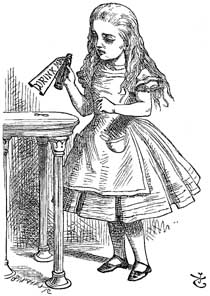
\includegraphics[width=0.5\textwidth]{images/alice.jpg}
    \caption[Alice mit Trinkflasche]{Um den Hals des Fläschchens war ein Zettel gebunden, mit den Worten "Trinke mich!" wunderschön in großen Buchstaben drauf gedruckt.
    \label{fig:Alice}}
\end{figure}

\subsection{Erster Unterabschnitt}

\subsubsection{Erster Unterunterabschnitt}

\lipsum[1-3]

\begin{table}[tb]
    \centering
    \begin{tabular}{ c | c c c }
        \toprule
                & Kaffee & Tee & Bier\\ 
        \midrule
        Morgens & 1 & 2 & 0\\  
        Mittags & 2 & 0 & 0\\ 
        Abends  & 0 & 3 & 1\\ 
        \bottomrule
    \end{tabular}
    \caption[Getränkeübersicht]{Übersicht über die Getränke, die an einem typischen Freitag  getrunken wurden.}
    \label{table:tab1}
\end{table}

